\documentclass[a4paper,12pt]{article}
\usepackage{latexsym}
\usepackage{array}
\usepackage{amsmath}
\usepackage{amsfonts}
\usepackage{amssymb}
\usepackage{bm}
\usepackage{color}
\usepackage{colortbl}
\usepackage{cite}
\usepackage{float}
\usepackage{graphicx}
\usepackage{ulem}
\usepackage{booktabs}
\usepackage[Symbol]{upgreek}
\usepackage{subfigure}
\usepackage{stfloats}
\usepackage{threeparttable}
\usepackage{theorem}
\usepackage{times}
\usepackage{dcolumn}
\usepackage{multirow}
\usepackage[boxed]{algorithm2e}
\usepackage{framed}

\newtheorem{theorem}{\bf Theorem}
\newtheorem{proposition}{\bf Proposition}
\newtheorem{lemma}{\bf Lemma}
\newtheorem{definition}{Definition}
\newtheorem{remark}{\bf Remark}


\setlength{\textheight}{245mm}
\setlength{\textwidth}{170mm}
\setlength{\topmargin}{-15mm}
\setlength{\oddsidemargin}{-5mm}
\setlength{\evensidemargin}{-5mm}
\flushbottom
\setlength{\parindent}{0pt}
\setlength{\baselineskip}{17pt}
\setlength{\parskip}{3mm}
\setlength{\columnsep}{8mm}
\renewcommand{\baselinestretch}{1.3}
\hyphenation{op-tical net-works semi-conduc-tor IEEEtran}
\DeclareGraphicsRule{.png}{eps}{.bb}{}
\allowdisplaybreaks[4]

\newcommand{\PreserveBackslash}[1]{\let\temp=\\#1\let\\=\temp}
\newcommand{\red}[1]{{\color{red}{#1}}}
\newcommand{\blue}[1]{{\color{blue}{#1}}}
\newcommand{\black}[1]{{\color{black}{#1}}}
\newcommand{\Authors}[1]{{\blue{{\textbf{Authors: }}{#1}}}}


\newenvironment{IEEEproof}{{\it Proof. }}{}
\newcolumntype{C}[1]{>{\PreserveBackslash\centering}p{#1}}
\newcolumntype{R}[1]{>{\PreserveBackslash\raggedleft}p{#1}}
\newcolumntype{L}[1]{>{\PreserveBackslash\raggedright}p{#1}}

\def \T {^{\mathsf{T}}}
\def \H {^{\mathsf{H}}}
\def \ri {{\rm i}}
\def \d {{\rm d}}
\def \tr {{\mathsf{tr}}\,}

\def\onecol{}

\begin{document}

\begin{center}
 {\Large\bf Electromagnetic Information Theory: Fundamentals, Modeling, Applications, and Open Problems}
\end{center}
\begin{center}
 {\Large\bf (Original paper ID: WCM-22-00602.R1)}
\end{center}
\begin{center}
 {\Large\bf Response Letter}
\end{center}
\begin{center}
Jieao Zhu, {\it Student Member,~IEEE}, Zhongzhichao Wan, {\it Student Member,~IEEE}, \\Linglong Dai, {\it Fellow,~IEEE},  M\'{e}rouane Debbah, {\it Fellow,~IEEE}, \\and H. Vincent Poor, {\it Life Fellow,~IEEE} 

\end{center}
\begin{center}
 {\Large\bf Response to Editor's Comments}
\end{center}


\textbf{Editor}: The review of the above manuscript submitted to IEEE Wireless Communications has been completed. The reviewers have recommended that major revisions be made to the manuscript. An acceptance decision will not be made until these revisions have been made and a second review has been completed. Please include detailed responses to the reviewers' comments.

\blue{
    {\bf Authors:}
    We would like to commence by thanking the editor and three professional reviewers for their valuable time in evaluating our submission. Your constructive comments and expert knowledge of the field have helped us to strengthen the manuscript significantly. We endeavored to address all the suggestions and comments, and our reflections are provided below in a point-to-point manner. We also indicate how our manuscript has been revised accordingly, and all the revisions have been highlighted in \red{red} color in the revised paper. Here, we would like to make a brief summary of the major revisions in the revised paper as below:
    \begin{enumerate}
        \item We have added necessary mathematical formulas to clarify the basic assumptions of each paragraph related to EIT. 
        \item We have carefully revised the figures and the corresponding descriptions to ensure that they are easy to understand. 
        \item We have provided new figures of numerical results to further illustrate the characteristics of the EIT mutual information.  
    \end{enumerate}
}

\blue{
    {\bf Authors}:
    Many thanks again for Editor's and all the Reviewer's valuable time and efforts to review this paper. Based on your constructive comments, we have already made a careful major revision of this paper, which is attached to the end of this letter. 
    \\
    \\
    Sincerely, 

    {\it The Authors}
}

\clearpage

%%%%%%%%%%%%%%%%%%%%%%%%%%%%%%%%%%%%%%%%%%%%%%%%%%%%%%%%%%%%%

\begin{center}
    {\Large\bf Response to Reviewer 2's Comments}
\end{center}

\textbf{Reviewer 2:}
In this revision, the reply from the authors is clear and reasonable. However, the paper has not been updated accordingly. 

1. In my previous review, a major concern is that the introduction does not clearly specify the potential deficiencies of existing information-theoretical models. To this end, the authors shall add more details to the paper to justify the new model, e.g., ``most of the existing models may over-estimate the MIMO channel capacity because they usually assume that 1) noises at different receiver antennas are independent, and 2) the power of noise is independent to the number of antennas''.

\blue{
    {\textbf{Authors: }} We appreciate the reviewer's overall supportive attitude to our reply. The paper has been updated according to your suggestions. In the revised version, we have clearly stated the potential deficiencies of existing information-theoretic models: 1) Ignoring the covariance of noise when the antennas become denser, and 2) Ignoring the dependence of noise power on the antenna density. The first statement is justified by the fact that, since the antennas are placed closer to each other, the EM mutual coupling effect will gradually contribute to the correlation of the measured noise signals. The second statement is justified by considering a spectrally white Brownian motion as the model for the noise process. When viewed in a large scale, the Brownian motion is cancelled out, and the average fluctuation is small, i.e., the noise for large-sized antennas are small. But when viewed in a very small scale, the thermal fluctuation becomes dominant, and thus the noise power increases [R1-2]. 
    
    
    {\bf References:}

    [R1] C. A. Balanis, {\it Antenna theory: analysis and design}, John Wiley \& Sons, 2016. 

    [R2] L. E. Reichl, {\it A modern course in statistical physics}, Americal Association of Physics Teachers, 1999. 


    \quad For you to check, the revisions are presented in the following box. 
    }

\begin{framed}
    {\bf Section I}

    \red{
        These assumptions will gradually become invalid when an ultradense MIMO, i.e., a continuous-aperture MIMO (CAP-MIMO), is considered. Specifically, the noise observed at each antenna will exhibit two distinct properties as the number of antennas increase. First, the noise will become correlated due to the strengthened electromagnetic (EM) mutual coupling. Second, the noise power will increase because of the exacerbated thermal fluctuation within small volumes. Both of these two effects will cause the traditional MIMO information-theoretic models to over-estimate the channel capacity, leading to mismatches between the system design and the actual wireless channel in the novel architectures beyond massive MIMO.
    }
\end{framed}

\textbf{Reviewer 2:}
2. For Fig. 2, variables $r$, $s$, $V_T$ must be defined. Since this article is a magazine paper, some more details shall be given, e.g., $J(s)$ and $E(r)$ are 3x1 vectors for 3D space, $G(r,s)$ is a 3x3 matrix, $E(r)$ can be obtained when $J(s)$ and $G(r,s)$ are given, etc.

\blue{
    {\bf Authors:}

    Thank you for pointing out the symbol problems. In the revised 
}


\textbf{Reviewer 2:}
In this paper, the authors briefly discussed the concept of Electromagnetic Information Theory (EIT). Specifically, in the first section, they introduced the main topic, i.e, EIT. Next, in Section 2, they explained the fundamentals of EIT, including (1) degree of freedom, (2) channel capacity, (3) Electromagnetic (EM) theory, and (4) random fields for EIT. In Section 3, the authors introduced modeling methodologies for EIT, including (1) continuous channel modeling, and (2) noise field modeling. In Section 4, they further discussed EIT analysis methods, such as (1) functional DoF, (2) channel DoF, and (3) mutual information and capacity analysis. Finally, the authors discussed some applications of EIT in Section 5 and open problems in Section 6, before concluding the paper in Section 7.

{\color{blue}{\textbf{Authors: } 
We appreciate the reviewer's concise summary of the key points of this paper. We have tried our best to revise the paper according to the reviewer's valuable comments, and our responses are provided in a point-to-point manner as below. 
}}


\textbf{Reviewer 2:}
Overall, the topic is fundamental and important to wireless communications. Nevertheless, the quality of the paper must be substantially improved. The major concerns are listed below.

1) In the introduction, the explanation of the potential deficiencies of existing information-theoretical models is very unclear. For example, what are the key issues of the discretization of transmitters/receivers, which is very common when modeling wireless channels? Does the discretization violate any physical laws? Does it overestimate or underestimate the information theoretical capacity of a wireless channel?


\blue{\textbf{Authors: } 
Many thanks for the reviewer's overall positive attitude on this magazine paper, and we are thankful to the reviewer for pointing out the limitations in the introduction part. We will commence by explaining why direct discretization, which is the foundation of the MIMO model, will inevitably lead to problematic results in evaluating the information-theoretic capacity of an electromagnetic (EM) communication system, especially when considering a superdense antenna array.

\quad The widely accepted MIMO channel model takes the form ${\bm y}={\bm H}{\bm x}+{\bm n}$, where ${\bm x}\in\mathbb{C}^{M}$ is the signals transmitted by the $M$-antenna transmitter, and ${\bm y}\in\mathbb{C}^{N}$ is the signals received by the $N$-antenna receiver. The MIMO channel is represented by ${\bm H}\in\mathbb{C}^{N\times M}$, and the noise vector ${\bm n}\sim \mathcal{CN}({\bm 0}_{N}, \sigma^2 {\bm I}_{N})$. The information-theoretic capacity is then expressed as 
\begin{equation}
    C = \log\det({\bm I}+\frac{1}{\sigma^2}{\bm H}{\bm C}_{\bm x}{\bm H}\H),
\end{equation}
where ${\bm C}_{\bm x}=\mathbb{E}\left[{\bm x}{\bm x}\H\right]$ is the covariance matrix of the transmitted signal ${\bm x}$, satisfying the transmit power constraint $\tr{\bm C}_{\bm x}\leq P_T$. The correctness of this classical MIMO model heavily relies on the following two discretization assumptions:
\begin{enumerate}
    \item The discrete\footnote{Here ``discrete'' means the noise values are random variables that are indexed by a discrete antenna index $n$} noise, i.e., the components of the noise vector ${\bm n}$, are uncorrelated for any pair of receive antennas. 
    \item The average discrete noise power $\sigma^2$ is a constant, which is independent of the number of transceiver antennas and the antenna spacing. 
\end{enumerate}
Note that the assumption (2) ensures an unchanged receive SNR $\gamma_{\rm R}=\mathbb{E}[{\bm y}\H{\bm y}]/(N\sigma^2)$ as the number of receive antennas $N\to\infty$ (but the receiving antennas are confined in a finite receive volume $V_{\rm R}$ [R1]). However, it can be numerically verified that as $N\to\infty$, the MIMO capacity $C$ will diverge to infinity, even if the channel model is given by the line-of-sight (LoS) Friis transmission formula: 
\begin{equation}
    [{\bm H}]_{mn}= \frac{\lambda}{4\pi r_{mn}}e^{-\ri 2\pi r_{mn}/\lambda},
\end{equation}
where $r_{mn}=|{\bm r}_m-{\bm r}_n'|$ is the geometric distance from the $m$-th transmit antenna to the $n$-th receive antenna, and $\lambda$ is the operating wavelength. This divergence of the system capacity contradicts the common belief that only a finite number of bits can be transmitted per unit time and unit bandwidth by the EM channel that connects a pair of given transmitter and receiver with confined volumes $V_{\rm T}$ and $V_{\rm R}$. 

\quad This contradiction occurs because the real-world EM systems do not follow the two discretization assumptions as are previously listed. (1) In real-world EM systems, the EM noise can be highly correlated, especially when the antenna spacing becomes smaller. This is because the EM coupling effect becomes more dominant when the antennas are placed closer to each other. A direct effect of this coupling on the mathematical model of the noise vector $\bm n$ is that the uncorrelated assumption is no longer valid, i.e., the noise exhibits a stronger spatial correlation. Mathematically, if this spatial correlation becomes stronger, the EM channel capacity will become lower. This is because a more correlated noise has a near-singular covariance matrix ${\bm C}_{\bm n}$, which decreases the MIMO capacity $C=\log\det(I+{\bm C}_{\bm y}{\bm C}_{\bm n}^{-1})$. In this way, recent results in [R1] have established a finite-valued capacity for this kind of EM channels, instead of an infinite value predicted by traditional discretized MIMO model as $N\to\infty$. (2) The noise power modeling problem is subordinate to the noise correlation modeling problem in (1), since the diagonal entries of a correlation matrix automatically gives the power of each noise random variable. 

\quad In summary, if we apply discretization to the EM systems in reality and try to reach a linear MIMO model, special attentions should be paid to the modeling of the noise vector ${\bm n}$. The discretization itself is correct, since any continuous function can be weakly approximated by its discrete counterpart (expressed by linear combinations of the $\delta$-functions) in functional analysis [R2], and this discretization does not violate any mathematical or physical principles. However, the discretized noise can exhibit a serious deviation from the uncorrelated standard Gaussian model, especially when the antenna spacing is much smaller than $\lambda/2$. Specifically, direct discretization of the noise will asymptotically overestimate the MIMO capacity. In the study of EIT, it is a key issue to reveal how the capacity behaves when the antenna spacing decreases. As a consequence, the widely applied discretization techniques and formulas should be re-investigated in order to reach a physically consistent conclusion when the transceivers approach the continuous case. 


{\bf References}

[R1] J. Zhu, Z. Zhang, Z. Wan, and L. Dai, ``On finite-time mutual information,'' in {\it Proc. 2022 IEEE Int. Symp. Inf. Theory (IEEE ISIT'22)}, Espoo, Finland, Jun. 2022. 

[R2] J. Muscat, {\it Functional analysis: An introduction to metric spaces, Hilbert spaces, and Banach algebras,} Springer, 2014. 

}

\blue{
    \quad Since the physical inconsistency caused by discretized noise covariance problem has not been widely noticed in the literature, in the revised version of this paper, we avoid the controversial discrete-continuous dilemma, and change the introduction part into a more general expectation on EIT. 
}

\begin{framed}
    {\bf Section I}
    
    \red{
    The past decade has witnessed the proliferation of the massive multiple-input multiple-output (MIMO)~[1] from a theoretical concept to a practical technology. Thanks to the ten-fold increase in transceiver antennas, the massive MIMO technology has triggered a significant performance improvement in 5G wireless communications. However, prevailing analysis and design procedures for massive MIMO are usually based on scalar-quantity, far-field~[2], discretized~[3], monochromatic, and other non-physically consistent assumptions, which will lead to mismatches between the system design and the actual propagation environment in the novel architectures beyond massive MIMO. Therefore, a theory that can model and analyze the real-world EM wireless information system with physically interpretable and mathematically reasonable assumptions is of interest, which motivates the research of EM information theory (EIT). }
\end{framed}

%%%%%%%%%%%%%%%%%%%%

\textbf{Reviewer 2:}
2) All the figures are confusing to readers.
2.1) There are many notations in Figs. 1, 2, 3, 4. However, they have not been clearly defined. 

2.2) In Fig.~1, there are four subfigures but it is unclear how they are related. For example, the two subfigures to the left are about a two-dimensional sub-space but it is not clear how they are relevant to the subfigures to the right.


\blue{
    {\bf Authors:} Thank you for pointing out these unclear parts in this paper. We have tried our best to fix these problems. The newly drawn figures are listed as follows, together with succinct descriptions of their contents. 

    \begin{figure}[!t]
        \centering 
        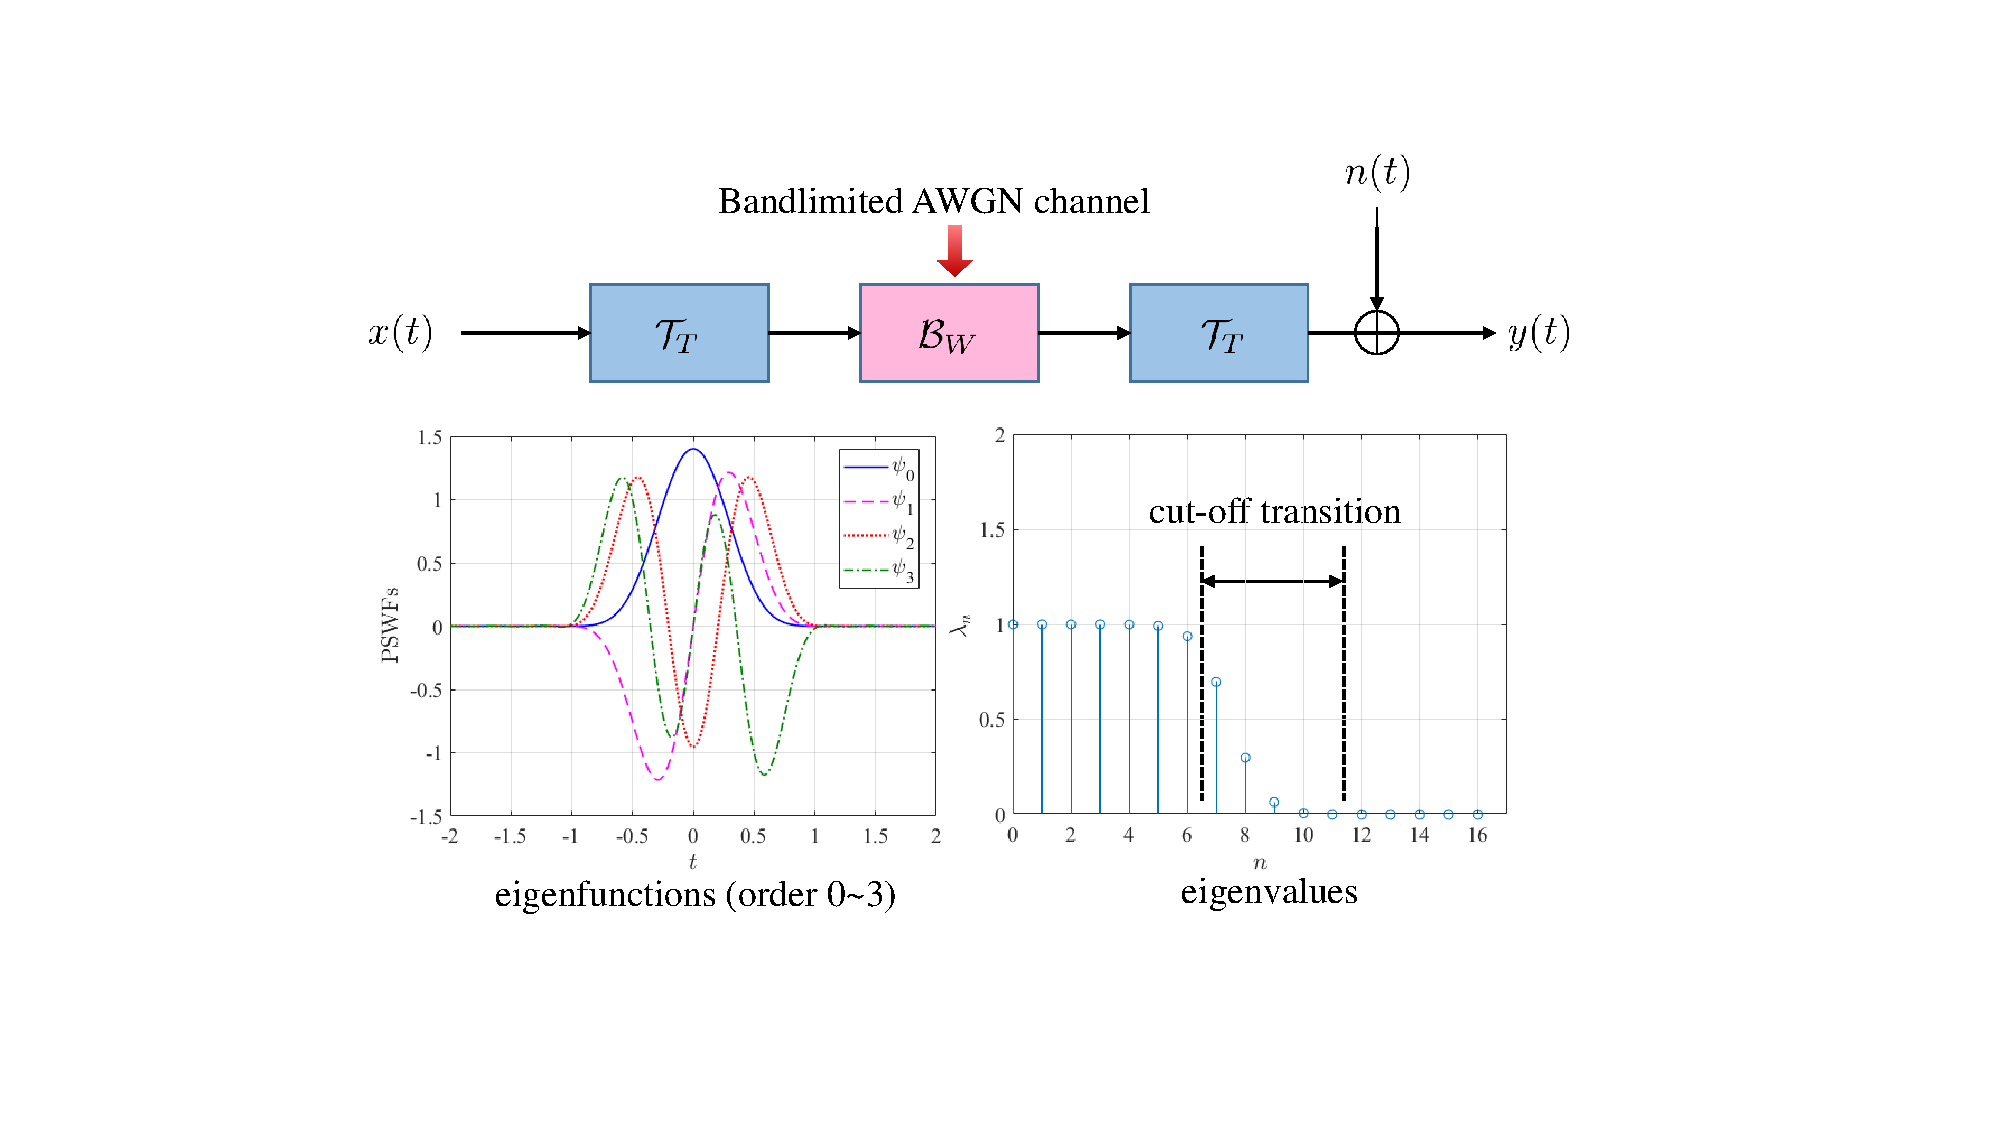
\includegraphics[width=0.8\linewidth]{../figures/PSWFs.pdf} 
        \caption{\blue{Example of the functional DoF: The bandlimited AWGN channel and its eigenmodes. The transmitted signal $x(t)$ is time-limited by the temporal truncation operator $\mathcal{T}_T$ before undergoing the $W$-bandlimited channel and a second truncation $\mathcal{T}_T$. The output of this channel $y(t)$ is then obtained by imposing an AWGN process $n(t)$. The eigenmodes of this linear system is given by the prolate spheroidal wave functions (PSWFs) $\{\psi_n\}_{n=0}^{\infty}$, with eigenvalues $\{\lambda_n\}_{n=0}^{\infty}$. In this figure, $T=2\,{\rm s}$, $W=2\,{\rm Hz}$, and thus the functional DoF of the recieved signal $y(t)$ is $2WT=8$. }}
        \label{fig:PSWF}
    \end{figure}
    
    \quad The contents of {\bf Fig.~1} are explained in the following. In Fig.~1, we describe how the functional DoF is evaluated by the classical example of the AWGN $W$-bandlimited channel. To evaluate the functional DoF of this channel, essentially we want to know how many ``different'' waveforms can be possibly observed at the output of this bandlimited channel within a given finite time interval $t\in[-T/2, T/2]$. 
    This degree of ``massiveness'' of such waveforms is translated into the Kolmogorov $N$-width $N_\epsilon$ of the bandlimited functional space ${\mathcal{B}_W}$, i.e., the minimum number of required basis functions to reconstruct any $f\in\mathcal{B}_W$ up to an error $\epsilon$.  
    The evaluation of $N_\epsilon$ can be fulfilled by finding a set of well-defined orthonormal basis functions $\psi_n(t)$ that spans the whole output set of this bandlimited $\mathcal{B}_W$, and translating the functional approximation problem in $L^2(-T/2, T/2)$ onto the equivalent coefficient approximation problem in the square-summable sequence space $\ell^2$ (Note that this translation map is an isometry from $L^2(-T/2, T/2)$ to $\ell^2$ due to the orthogonality of the chosen basis functions). A refined analysis on these orthonormal basis functions has proved that they are in fact prolate spheroidal wave functions (PSWFs), which are shown in the newly drawn {\bf Fig.~1}. Further mathematical analysis also shows that, the Kolmogorov $N$-width $N_\epsilon$ is intrinsically equal to the number of channel gains $\lambda_n$ that exceeds a predetermined threshold $\epsilon$, where the channel gains $\lambda_n$ are defined to be the gain of this $W$-bandlimited AWGN channel when the $n$-th PSWF is input into the channel. 


    In the revised version of this paper, we have addressed these issue as:

}

\begin{framed}
    {\bf Section II-A}

    \red{
        By contrast, in the information theory community, the DoF has a mathematically rigorous definition that is firmly rooted in the spectral theory in functional analysis. 
        Generally, if a normed functional space $\mathcal{X}$ contains an $N$-dimensional subspace $\mathcal{X}_N$ such that any function $f\in\mathcal{X}$ can be ``well-approximated'' by some $\hat{f}\in\mathcal{X}_N$, then it is reasonable to claim that the space $\mathcal{X}$ has an essential DoF of $N$.  
        An inspiring and important example would be evaluating the DoF of a waveform channel bandlimited to $[-W, W]\, {\rm Hz}$, as is shown in Fig.~1. Equivalently, we want to know how many real numbers can be communicated per unit time through this $W$-bandlimited channel. 
        Slepian solved this problem by collecting all the $W$-bandlimited signals together into a functional space $\mathcal{B}_W$, and asking at least how many coefficients $\{x_n\}_{n=1}^{N_\epsilon}$ are needed to approximate an arbitrary $f(t)\in \mathcal{B}_W$ up to a precision of $\epsilon$, i.e., $\|f(t)-\sum_{n=1}^{N_\epsilon}x_n\phi_n(t)\|/\|f\|\leq \epsilon$.
        This minimum number of coefficients $N_\epsilon$ is called the Kolmogorov $N$-width $N_\epsilon(\mathcal{B}_W)$ of the functional space $\mathcal{B}_W$ under given norm $\|\cdot\|$. Since data transmission usually takes place within a finite time interval $[-T/2, T/2]$, the norm is chosen to be $L^2(-T/2, T/2)$. Then, the conclusion is that $N_\epsilon=2WT+\mathcal{O}(\log (WT))$~[4] holds for any given $\epsilon>0$. 
        This means that the $W$-bandlimited channel can essentially transmit $2WT$ real numbers within time $T$. 
        In this case, the optimal basis waveforms $\psi_n(t)$ are prolate spheroidal wave functions (PSWFs), which are shown in Fig.~1. Note that the functional DoF of the received signal $y(t)$ is determined by evaluating the largest $n$ before the eigenvalues $\lambda_n$ exhibit a cut-off transition behavior. 
    }

\end{framed}


\textbf{Reviewer 2:}
2.3) In Fig.~2, the input, output, and channel must be specific and related. For instance, for the LTI system, the authors must specify whether the n is in the time or frequency domain. Then, the output $Y(n)$ shall be the product of $X(n)$ and $H(n)$ if they are in the frequency domain.

\blue{
    {\bf Authors:} Many thanks for the reviewer's constructive suggestions. In the original version of this Fig.~2, we intended to compare between the linear time-invariant (LTI) systems that are widely adopted as discrete-time channel models and the linear space-invariant systems that are not familiar to the communications society. For the LTI systems, the channel input is a discrete time-domain complex-valued sequence $x(n)$ that are usually generated by IQ modulation. The channel is usually characterized by a complex time-domain impulse response $h(n)$, which is the frequency-shifted version of the frequency-band electromagnetic impulse response. The channel output $y(n)$ is the received sequence, which is usually the convolution of $x(n)$ and $h(n)$ plus the noise. The convolution operation originates from the linear property and the temporal shift-invariant property of the wireless channel. 

    \quad Similar to the time-domain LTI systems, in electromagnetic information theory (EIT), the electromagnetic channels can be modeled by space-domain LSI systems. Strictly speaking, this requires the wireless propagation environment to be invariant under spatial translation, and the requirement is only satisfied in free-space propagation. However, for future high-frequency wireless applications, the real-world propagation channels are dominated by line-of-sight (LoS) paths, and thus can be well-approximated by the free-space LSI systems.  

    \quad The detailed description of the LSI systems is provided as follows. In Fig.~2, a narrowband wireless transmission system is considered, where the transmitter is confined to the spatial region $V_{\rm T}$, and the receiver is confined to the spatial region $V_{\rm R}$. The transmitter generates a source current distribution ${\bm J}({\bm s})\in\mathbb{C}^3 \;{\rm unit:[A/m^2]}$, which induces a received electric field ${\bm E}({\bm r})\in\mathbb{C}^3\;{\rm unit:[V/m]}$ at the receiver via the electromagnetic channel ${\bm G}({\bm r}, {\bm s})\in\mathbb{C}^{3\times 3}\,{\rm unit:[\Omega/m^2]}$ (or Green's function). The input-output relationship is given by 
    \begin{equation}
        {\bm E}({\bm r})=\int_{V_{\rm T}} {\bm G}({\bm r}, {\bm s}){\bm J}({\bm s}){\rm d}{\bm s}, 
    \end{equation}
    and the noisy received field is ${\bm Y}({\bm r}) = {\bm E}({\bm r})+{\bm N}({\bm r})$. With the free-space isotropic propagation assumption, the Green's function ${\bm G}$ is expressed as 
    \begin{equation}
        \begin{aligned}
            {\bf{G}}({\bf{r}},{\bf{s}}) &= \frac{{\rm j}\kappa_0 {Z_0}}{{4\pi }} \left( {{\bf{I}} + \frac{{{\nabla _{\bf{r}}}\nabla _{\bf{r}}^{\rm{H}}}}{{{\kappa_0 ^2}}}} \right) \frac{{{e^{{\rm{j}}\kappa_0 \left\| {{\bf{r}} - {\bf{s}}} \right\|}}}}{{\left\| {{\bf{r}} - {\bf{s}}} \right\|}}  \\
            &= \frac{{\rm j}\kappa_0 {Z_0}}{{4\pi }}\frac{{{e^{{\rm{j}}\kappa_0 \left\| {{\bf{r}} - {\bf{s}}} \right\|}}}}{{\left\| {{\bf{r}} - {\bf{s}}} \right\|}}\Bigg[\left( {{\bf{I}} - {\bf{\hat p}}{{{\bf{\hat p}}}^{\rm{H}}}} \right) \\&~~+ \frac{{\rm j}}{2\pi \left\| {{\bf{r}} - {\bf{s}}} \right\| /\lambda}\left( {\bf I}-3{\bf{\hat p}}{{{\bf{\hat p}}}^{\rm{H}}} \right) \\&~~-\frac{1}{(2\pi\left\| {{\bf{r}} - {\bf{s}}} \right\|/\lambda )^2 }\left( {\bf I}-3{\bf{\hat p}}{{{\bf{\hat p}}}^{\rm{H}}}  \right) \Bigg] [{\rm \Omega}/{\rm m}^2], 
            \label{Green}
        \end{aligned}
    \end{equation}
    where ${\bm p}={\bm r}-{\bm s}$, $\hat{\bm p}={\bm p}/\|{\bm p}\|$, $\kappa_0=\omega_0\sqrt{\mu\epsilon}$ is the propagation constant, and $Z_0$ is the intrinsic impedance of a vacuum. 

    \quad Note that in order to emphasize the functional nature of the source current ${\bm J}({\bm s})$ and the received electric field ${\bm E}({\bm r})$, we treat them as square-integrable ($\mathcal{L}_2$) functions living on their own domains of definition.  In the revised paper, we have clarified the definitions of the input-output relationship as follows. 

}

\begin{framed}
    {\bf Section III-A}

    \red{In this part, we will discuss the channel models in EIT, which describe the EM channel by a bounded linear operator $T$ that maps the source current distribution ${\bm J}({\bm s})\in\mathcal{L}^2(V_{\rm T})$ to the noiseless received field ${\bm E}({\bm r})\in\mathcal{L}^2(V_{\rm R})$. 
    Note that to model a traditional narrowband MIMO channel, a matrix with complex-valued entries ${\bm H}:\mathbb{C}^M\to\mathbb{C}^N$ is usually utilized, where each entry represents the complex channel between a pair of transceiver antennas. 
    This channel model is, in essence, spatially discrete. 
    However, in EIT, it is reasonably assumed that one can measure the field at an arbitrary point inside the receiver region, where the precision of such measurement is subject to some physical noise limits. This leads to the assumption of EIT that the transceivers operate in a continuous functional space $\mathcal{L}^2(V_{\{{\rm T, R}\}})$.  }
\end{framed}

\textbf{Reviewer 2:}
2.4) In Fig.~2, the authors shall try to use the continuous system to avoid confusing readers because discrete and discretization have been used in the first section to distinguish classical IT and EIT.

\blue{
    {\bf Authors:}

    \quad As is pointed out by the reviewer, the figure (Fig.~\ref{fig:LTI_LSI_new} in this response, which corresponds to Fig.~2 in the magazine paper) is somewhat confusing, since discrete and discretization have already been used in the first section to distinguish between classical IT and EIT. We agree with the reviewer that, in Fig.~2 there is no need to stress the difference of IT and EIT again. So we clarify the motive of Fig.~2 as follows.
    
    \begin{figure}[htbp]  
        \centering
        \begin{minipage}[t]{0.45\linewidth}  
            \centering  
            \setlength{\belowcaptionskip}{-0.1cm} 
            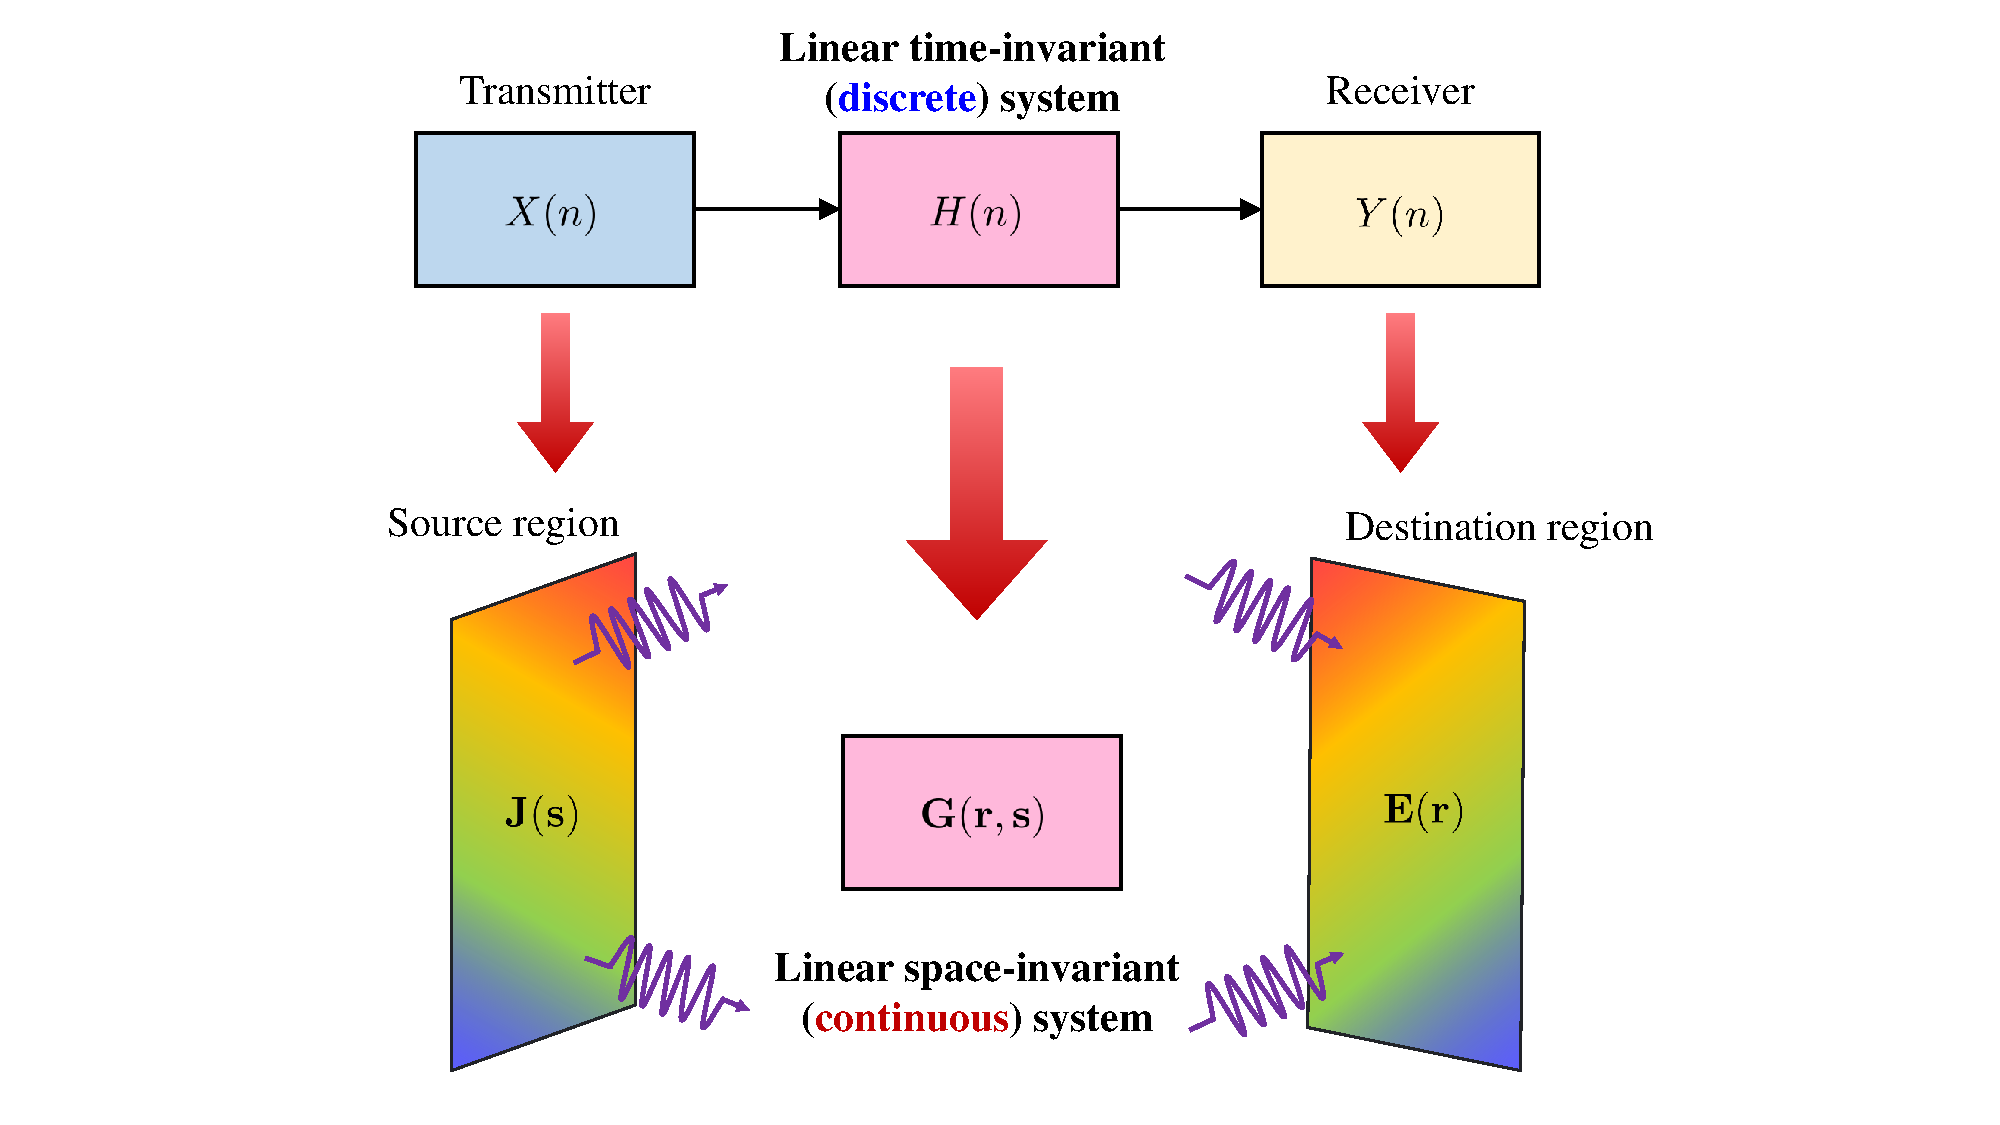
\includegraphics[width=7cm]{../figures/LTI-LSI-new.pdf}  
            \caption{\small Old version of this figure. }  \label{fig:LTI_LSI_new}
        \end{minipage}
        \begin{minipage}[t]{0.45\linewidth}  
            \centering  
            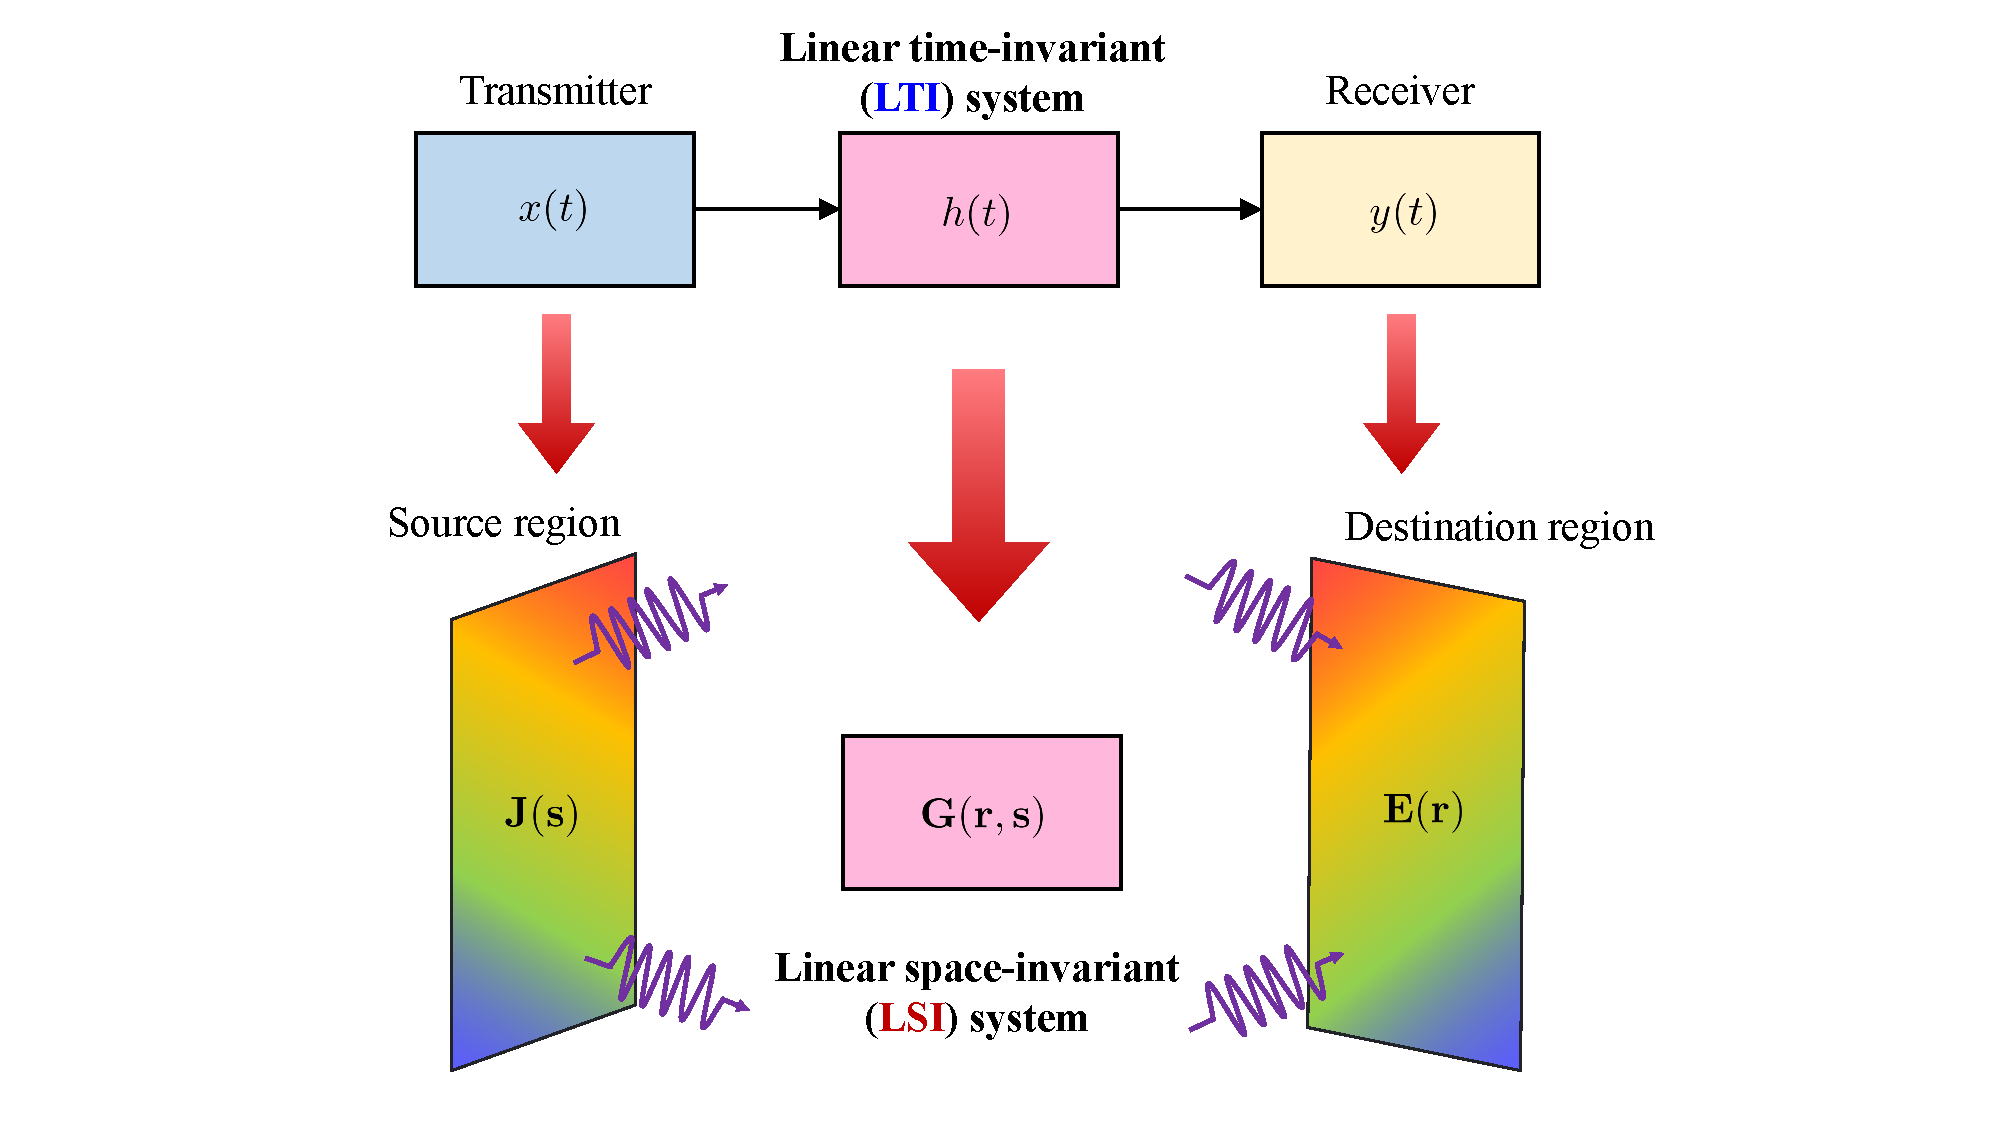
\includegraphics[width=7cm]{../figures/LTI-LSI-new-v1.pdf}  
            \caption{\small Updated version of this figure. }  \label{fig:LTI_LSI_new-v1}
        \end{minipage}  
    \end{figure}


    \quad In fact, this figure is intended for emphasizing the analogous connection between the discrete-time linear time-invariant (LTI) model in classical IT and the continuous-space linear space-invariant (LSI) model in EIT. The connection lies in the fact that, the free-space isotropic electromagnetic impulse response is both linearly invariant in the time domain and linearly invariant in the space domain. To address the confusion, in the revised version of this figure, we have replaced the discrete time index $n$ with the continuous time index $t$, so as to strengthen the analogy of LTI-LSI systems instead of the discrete-continuous difference. 

    We have also clarified this analogy in the following revised paragraphs of this paper, which are shown in the following box: 
}


\begin{framed}
    {\bf Fig.~2 Caption}

    \red{In analogy with linear time-invariant systems described by a time-domain impulse response $h(t)$ in classical information theory, the EIT model is based on linear space-invariant systems described by the Green's function ${\bm G}({\bm r}, {\bm s})$.}

    {\bf Section II-C}

    \red{In wireless communications, to describe the EM response at the receiver induced by the transmitted wave at the transmitter, Green's function ${\bm G}({\bm r}, {\bm s})$ is usually introduced as the spatial impulse response of EM systems~[6], with ${\bm J}({\bm s})$ being the transmitted source current, and ${\bm E}({\bm r})$ being the received electric field, as is shown in Fig.~\ref{fig:LTI_LSI_new}. Since the electric and magnetic field vectors are all three-dimensional time-varying vectors, to describe the mapping between two vectors, Green's function must take the form of a dyadic-valued function. 
    Note that EM theory is a deterministic theory built on partial differential equations and the knowledge of all surroundings, so Green's function is uniquely determined by the boundary conditions of EM problems.
    As a result, pure EM theory cannot capture the random nature that arises in wireless communications.  }
\end{framed}



\textbf{Reviewer 2:}
3) In Section 3 and Section 4, all discussions about modeling are difficult for readers. To this end, the main assumptions must be clearly illustrated at the beginning and a few equations may be necessary to understand the discussions in Section 3 and Section 4.

\blue{
    {\bf Authors:} Many thanks for the reviewer's suggestion. In order to facilitate understanding, we have carefully revised the current version of this magazine paper. For you to check, the modifications are provided in the following boxes in a pointwise manner. 
}

\blue{
    \quad In the beginning of {\bf Section III-A}, we have clarified the main assumptions of the EIT system model by comparing the EIT channel operator with the traditional MIMO channel matrix. 
}

\begin{framed}
    {\bf Section III-A}

    \red{In this part, we will discuss the channel models in EIT, which describe the EM channel by a bounded linear operator $T$ that maps the source current distribution ${\bm J}({\bm s})\in\mathcal{L}^2(V_{\rm T})$ to the noiseless received field ${\bm E}({\bm r})\in\mathcal{L}^2(V_{\rm R})$.   
    Note that to model a traditional narrowband MIMO channel, a matrix with complex-valued entries ${\bm H}:\mathbb{C}^M\to\mathbb{C}^N$ is usually utilized, where each entry represents the complex channel between a pair of transceiver antennas. 
    This channel model is, in essence, spatially discrete. 
    However, in EIT, it is reasonably assumed that one can measure the field at an arbitrary point inside the receiver region, where the precision of such measurement is subject to some physical noise limits. This leads to the assumption of EIT that the transceivers operate in a continuous functional space $\mathcal{L}^2(V_{\{{\rm T, R}\}})$. }

\end{framed}

\blue{
    \quad In the middle of {\bf Section III-A}, we have emphasized the connection between the EIT operator channel $T$ and the MIMO matrix channel ${\bm H}$ by mathematical formulas, using the standard and simple symbols in Hilbert spaces. 
}

\begin{framed}
    {\bf Section III-A}

    \red{To ensure compatibility with discrete MIMO channel modeling, the connection between the entries of ${\bm H}$ and the transceiver antenna modes are usually assumed to be ${\bm H}_{qp}=\langle\varphi_q|T|\phi_p \rangle$, where $\phi_p$ and $\varphi_q$ are the $p$-th and $q$-th operating modes of the transmit and receive antennas, respectively. Thus, modeling the EM channel by a bounded linear operator $T$ is mathematically consistent with the existing matrix modeling. }
\end{framed}

\blue{
    \quad In {\bf Section III-B} (EIT Noise Field Modeling), we have accurately clarified the difference between the noise assumptions in IT and those in EIT by simple terms and the corresponding mathematical symbols. 
}

\begin{framed}
    {\bf Section III-B} 

    \red{
        In classical information theory, the noise is usually modeled by a time-domain additive white Gaussian noise (AWGN) with a constant power spectral density $n_0/2$. Thus, its projection coefficients onto any orthonormal basis are independent and of equal power $n_0/2$, which simplifies theoretical analysis. 
        Similarly, in EIT, the noise is usually modeled as a spatial AWGN with flat wavenumber PSD. This spatial AWGN implies that the additive noises at any disjoint small spatial regions $V_1, V_2$ are independent and identically distributed (i.i.d.) complex Gaussian random variables, whose variances are proportional to the volumes $\mu(V_1), \mu(V_2)$ of the small regions. Although the AWGN model facilitates theoretical analysis, the white spectral assumption is problematic, since it causes an unbounded noise power. 
    }
\end{framed}

\blue{
    \quad To explain the theoretical techniques for evaluating the functional DoF in EIT, we have added the transform formulas for electric fields, and the asymptotic spatial bandwidth conclusions in the formula form. 
}

\begin{framed}
    {\bf Section IV-A}

    \red{The functional DoF of a scattered EM field ${\bm E}({\bm r})$ can be analyzed in the transform domain ${\bm E}({\bm k}) = \mathcal{F}^3[{\bm E}({\bm r})]({\bm k})$, i.e., the wavenumber domain. Resembling the bandlimited signals in the time-frequency domain, the radiated EM fields also exhibit the wavenumber-limited property in the space-wavenumber domain. 
    Thus, it can be easily proved that a half-wavelength sampling suffices to asymptotically reconstruct an arbitrary EM field up to any given precision $\epsilon$ as the receiving region $\mu(V_{\rm R})\to\infty$, i.e., the EM DoF is at most proportional to the number of half-wavelength grids in the receiver region. }

    {\bf Section IV-A}

    \red{
    To describe such a phase change, the authors of~[9] introduced the spatial bandwidth $W$ to describe the degree of wavenumber-limitedness. 
    It is proved that for electromagnetic sources confined to a sphere of radius $a$, the spatial bandwidth satisfies $W\leq \sqrt{2}\beta a$, where $\beta$ is the propagation constant of the time-harmonic EM fields. 
    The functional DoF of the received field is thus proportional to $W$ and the length of the observation region. }
\end{framed}

\blue{
    \quad We have clarified the eigenmode decomposition techniques (operator SVD) in the evaluation of the electromagnetic channel DoF. 
}

\begin{framed}
    {\bf Section IV-B}

    \red{As is defined in Subsection~II-A, the channel DoF represents the maximum number of independent parallel channels that can be used to transmit information. 
    Similar to the SVD decomposition of matrices, the DoF of a LoS EM channel can be solved by expanding the channel operator $T$ onto a series of orthogonal sub-channels: $T=\sum_n \sigma_n |\psi_n\rangle\langle\phi_n|$, and counting the number of channel gains $\sigma_n$ that exceed a certain threshold $\epsilon$. 
    Specifically, in the scenario where a pair of coaxial square transceivers are employed as transmit and receive antennas, the LoS channel operator $T$ is given by the free-space Green's function ${\bm G}({\bm r}, {\bm s})$, and the corresponding eigenvalue problem can be approximated by the standard Slepian's concentration problem~[10]. In this case, the channel eigenmodes $\psi_n$ and $\phi_n$ are proved to be well-approximated by prolate spheroidal wave functions $\varphi_n(x)$.   
    Through this approach, the DoF of LoS channel model has been approximately derived to be proportional to the product of the area of the transceivers~[10], [11]. }
\end{framed}


{\color{blue}{\textbf{Authors: } 
Many thanks again for your valuable time and efforts to review this paper. 
\\
\\
Sincerely, \\
{\it The Authors }
}}

\clearpage 


\end{document}
